% - Theoretical introduction and motivation
% - Idea behind the ATLAS experiment and search
% - Future use of this information

\section{Introduction} % (non-mathematical)
% Breif introduction to the Standard Model and Gauge Symmetries 

% Motivation for spontaneous symmetry breaking / the higgs mechanism

% The current status of the Higgs search

% Motivation for searching for H->Zg

% The ATLAS experiment and the form of the measurement, 
% i.e. how and what is measured

Elementary particle physics addresses the question, `What is the world made of?' 
at the most fundamental level, i.e. on the smallest scale of size. 
One could easily imagine a world where the elementary building blocks of 
nature come in a vast variety of shapes and sizes. Just think of the multitude of 
parts that work together to make up an ordinary car. Remarkably this is not
the case. The tiniest chunks of nature come in a small number of different types
(electrons, quarks, photons, and so on), which are replicated in astronomical
quantities to form our macroscopic world. This is not the whole story.
Not only is elementary particle physics concerned with identifying the various 
fundamental actors of nature, but also how these actors interact amongst each other.
It is during this investigation that the familiar forces of nature make their
appearance. This paper is concerned with measuring both of these phenomena through 
a search for a new particle known as the Higgs boson as well as an investigation of
how this particle interacts with two other important actors: the photon and the 
$Z$ boson.

The current answer to the question of what the world is made of is displayed in 
Figure~\ref{fig:sm} and is known as the Standard Model. This table is reminiscent
of the periodic table developed by chemists to explain the various atoms
found in nature. A surprising property of the Standard Model is that it consists
of only 16 different particles. There are six quarks, shown in purple, which
are the building blocks of the familiar nucleons, i.e. the proton and neutron.
Another six particles known as leptons, marked in green, include one of
the most familiar fundamental particles, the electron, 
which is responsible for the operation of most household circuits. And
finally there are the four gauge bosons highlighted in red, which are of the 
greatest relevance to the measurement presented in this paper.
The gauge bosons are responsible mediating three 
out of the four fundamental forces in nature: the electromagnetic, strong, and 
weak interactions
\footnote{As of now, theorists have been unable to incorporate the 
gravitational force, a pervasive component of the macroscopic world,
into the current theory of particle physics.}.

\begin{figure}[htbp]
    \centering
    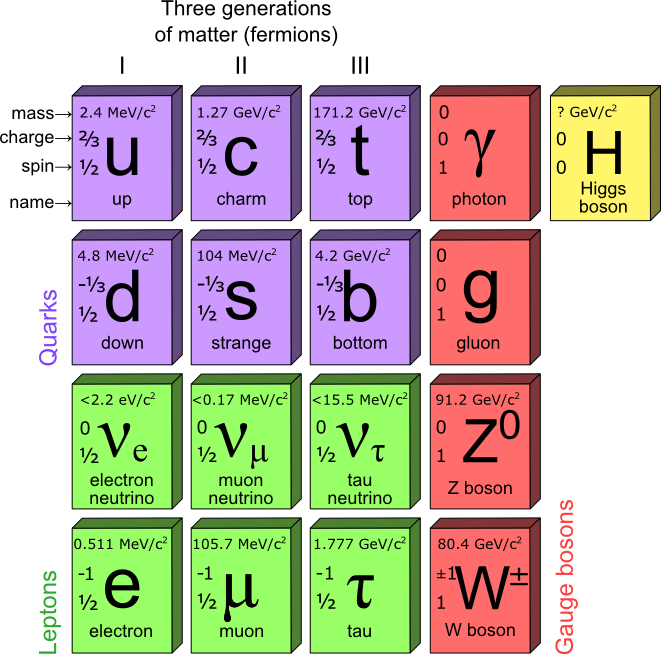
\includegraphics[scale=0.4, angle=0]{./figures/StandardModelPNG}
    \caption{A table summarizing the particles described by the
    Standard Model of particle physics. The Standard Model encompasses
    three generations of quarks and leptons as well as four force carrying
    bosons.}
    \label{fig:sm}
\end{figure}

The Higgs boson is an essential component of the Standard Model and plays
an important role in the predictive power of the theory. Like much of modern
physics, the Standard Model relies heavily on the symmetries of nature. Just
as concepts such as conservation of momentum and energy can be tied to the 
fact that a system is symmetric under translations in space and time\footnote{
This result is known as Noether's Theorem and can be attributed to the 
brilliant German mathematician Emmy Noether.}, much of the mathematical 
framework of the Standard Model is based on internal symmetries 
known as gauge symmetries. In fact there are three gauge symmetries found
in the Standard Model\footnote{ In group theoretic language the symmetries of
the Standard Model can be written as $SU(3) \times SU(2) \times U(1)$.} 
each of which predicts a force carrying particle that mediates one of the 
aforementioned interactions of nature. The photon mediates the 
electromagnetic interaction. The massless gluon is responsible for the strong 
interaction, which binds quarks together to form protons and neutrons.
And finally, the weak interaction, which causes radioactive decays, 
is mediated by the massive \WBosons and \ZBoson bosons. The problem with all 
of this symmetry is that it predicts that the weak nuclear force is a long
range force, something which is not observed in nature. The reason for this
discrepancy can be traced back to the fact that the \WBoson and \ZBoson bosons are
not massless particles, but have a mass of roughly 80 and 90 GeV respectively. 
In addition, these internal gauge symmetries also predict that other 
fundamental particles, such as the electron, are massless. In order to solve
this apparent predicament one needs to introduce a mechanism that keeps the
equations that govern the Standard Model's behavior symmetric, but allows for
some asymmetric lowest energy states, i.e. 'ground states'. 
This is accomplished with a theoretical mechanism known as spontaneous
symmetry breaking or in this special case the Higgs mechanism.

On July 4th, 2012 the ATLAS and CMS collaborations both announced the 
discovery of a particle consistent with the 
Standard Model Higgs boson~\cite{ATLAS_Higgs,CMS_Higgs}, indicating that
the discovery of the mechanism behind spontaneous symmetry breaking in the
Standard Model may be at hand. In addition, the ATLAS experiment measured 
this Higgs-like boson's mass to be close to 125 GeV~\cite{ATLAS_Higgs_Dec12}.
This measurement is only the beginning of a challenging program of `Higgs
identification' through which the consistency of this new boson with the SM
Higgs will be verified or disproved. For this reason it is now becoming
increasingly important to measure the properties of this new scalar particle
as well as its rate of decay for the largest number of experimentally
viable decay channels. These analyses could result in tension with the SM
Higgs prediction, for instance the rate of one or more measured decay channels
may differ from the SM prediction. The simplest mechanism for such a scenario
is an enhancement/suppression in loop-induced decays
\footnote{A loop means that particles of any mass can instantly materialize and 
then disappear during the decay process. The brief-lived virtual particles
are usually $W$ bosons, but other particles with similar behavior can enter
the loop, including many beyond the Standard Model particles. This makes decays 
involving loops very sensitive to new physics at high masses.}
that are naturally sensitive to couplings to new virtual particles, 
for instance the decay \HToZg presented in this paper. 
This would thus be evidence for Beyond the Standard Model (BSM) physics.

The main decay modes being probed in the searches
presented during the July 4th announcement are the $H \to \gamma\gamma$ channel,
the $H \to WW^* \to 2\ell2\nu$ channel and the 'golden channel',
$H \to ZZ^* \to 4\ell$. However, little attention has been paid to the 
$H \to Z\gamma \to \ell^+\ell^-\gamma$ channel
despite the fact that its event rate is comparable to that of the golden channel 
for a 125 GeV Standard Model Higgs boson. The main reason for this is 
the low branching ratio for $Z \to \ell^+\ell^-$, the
probability that a $Z$ boson will decay into two leptons, 
makes the $Z\gamma$ channel statistically limited. 
Although, the background rate, the number of non-interesting physics processes
that contaminate the process of interest, of the $Z\gamma$ channel is higher than
that of the $ZZ^* \rightarrow 4\ell$ channel
there are a few important properties that make a study of the $Z\gamma$ channel 
compelling: 
1) all final state particles can be measured well with the ATLAS detector;  
2) the Higgs mass could be measured from the total invariant mass spectrum; 
3) the spin of the Higgs can be studied by analyzing the angular distribution 
of the decay products, and 
4) this channel can be used for setting limits on the Higgs coupling constants.
In addition, the ratio of $\gamma\gamma$ to $Z\gamma$ branching ratios can
be used to discriminate between certain models of 
new physics~\cite{Zg_newPhy_1,Zg_newPhy_2, Zg_newPhy_3}.
All of these measurements will help to identify this new particle sitting
close to 125 GeV as a Standard Model Higgs boson or something more exotic.

% re-write this with my own words....
This report documents the measurements of the \HToZg production rate observed
using data from $pp$ collisions provided by the LHC. In the following, the
theory behind the \HToZg decay is discussed in Section~\ref{sec:theory},
the ATLAS detector is described in Section~\ref{sec:atlas}, and the signal
and backgrond simulation samples used in the analysis are presented in
Section~\ref{sec:sigbkg}. The event selection criteria are described in 
Section~\ref{sec:event}. A comparison between the selected data sample and
the simulation is presented in Section~\ref{sec:compare}. The discrimination
between signal and background events is performed by means of an unbinned
maximum likelihood fit, and the estimated signal yield is compared to the one 
predicted by the Standard Model. The properties of the signal, in terms of
the expected yields and the signal model used for the fit are described
in Section~\ref{sec:signal}, while the choice of the background model adopted
in the fit is motivated in Section~\ref{sec:background}. After a description of
the systematic uncertainties in Section~\ref{sec:sys}, Section~\ref{sec:results}
presents the results of the combined analysis of the 7 and 8 TeV datasets.
